\documentclass[a4paper, 11pt]{article}

\usepackage[french]{babel}
\usepackage[utf8]{inputenc}
\usepackage[T1]{fontenc}
\usepackage{graphicx}
\usepackage[colorinlistoftodos]{todonotes}
\usepackage{listings}
\usepackage{lscape}

\graphicspath{{img/}}

\title{\Huge{SmartProjector}}

\author{BRANGER Mathias, HABLOT Jules}

\date{\today}

\begin{document}

\maketitle

\begin{figure}
	\centering
	
\includegraphics[width=1\textwidth]{polytech.jpg}
\end{figure}

\clearpage

\tableofcontents

\clearpage

%\begin{figure}[!h]
%	\centering
%	\includegraphics[width=1\textwidth]{sphere_initiale.png}
%	\caption{Sphere initiale}
%\end{figure}

%\begin{figure}[!ht] \centering
%        \begin{minipage}[t]{6cm}
%                \includegraphics[width=1\textwidth]{sphere_damier.png}
%                \caption{\newline Sphère avec une texture en damier}
%        \end{minipage} 
%        \begin{minipage}[t]{6cm}
%                \includegraphics[width=1\textwidth]{sphere_terre.png}
%                \caption{\newline Texture de la terre avec vue sur le pôle sud}
%        \end{minipage}
%\end{figure}

\section{Introduction}

De nos jours, les présentations sur vidéoprojecteur sont de plus de plus courantes. Néanmoins, la technologie sans fil dans ce domaine n'est pas encore très développée. Par exemple, dans notre école, des vidéoprojecteurs sont présents dans toutes les salles mais il faut s'y connecter par câble VGA. Ce type de port était très répandu sur les anciens et volumineux ordinateurs portables, mais il est désormais trop gros pour être mis sur nos ultras-books. Il nous faut donc acheter des adaptateurs et ne pas les oublier. De plus, nous sommes parfois confrontés à des problèmes de connectique : le câble VGA sont mal branché à la prise murale, les embouts sont détruits par des élèves malveillants…

\section{Notre projet}

Nous apportons la solution pour régler tous ces problèmes. Nous proposons une application qui sera disponible sur toutes les plateformes et qui permettra une connexion wifi entre les ordinateurs portables des utilisateurs et le vidéoprojecteur. Les utilisateurs pourront se connecter seuls ou à plusieurs en même temps sur le vidéoprojecteur. Des élèves se partageront l'écran, mais un professeur aura, lui, accès à plus de fonctionnalités que les élèves. Il pourra notamment choisir l'écran à afficher sur le vidéoprojecteur.

\section{Technologies utilisées}

Nous avons commencé par rechercher d'éventuelles solutions sur internet afin de ne pas reproduire un projet déjà abouti et fonctionnel. 

Nous nous sommes ensuite interrogés sur des technologies existantes qui pourraient nous être utiles par la suite. Nous avons aussi demandé de l'aide à des professeurs pour nous conseiller certains types de technologies à utiliser. Ainsi, nous avons entendu parler de \textbf{WebRTC}, \textbf{HTML5}, \textbf{GStreamer} concernant les frameworks de gestions de flux. 

\begin{figure}[!ht] \centering
        \begin{minipage}[t]{3.5cm}
                
\includegraphics[width=1\textwidth]{HTML5_logo.png}
        \end{minipage} 
        \begin{minipage}[t]{3.5cm}
                
\includegraphics[width=1\textwidth]{logo_webrtc.png}
        \end{minipage}
         \begin{minipage}[t]{4cm}
                
\includegraphics[width=1\textwidth]{Gstreamer_logo.png}
        \end{minipage}
\end{figure}


Après analyse de \textbf{HTML5} et de \textbf{WebRTC} nous avons décidé d'écarter ces technologies car elles ne répondaient pas à nos attentes. En effet, nous devions passer par un navigateur pour partager un flux vidéo et nous n'arrivions pas à partager le flux vidéo de notre écran.

Nous devions aussi choisir une librairie graphique compatible avec toutes les plateformes.

\subsection{GStreamer}

Nous nous sommes intéressés, suite aux conseils de Jérôme Maisonasse, au framework GStreamer. Il s'agit d'une librairie C/C++ pour faire du transfert de flux. Sa prise en main était simple : nous pouvions tester les différentes fonctionnalités grâce à une ligne de commande. Nous nous sommes donc très vite décidé à utiliser ce framework car il correspondait à toutes nos attentes : nous pouvions facilement splitter un écran en 4 et recevoir 4 flux simultanément (dont certains provenant du réseau). Néanmoins, nous avons été confrontés à un problème : la gestion dynamique des flux. En effet, lors de la connexion (ou déconnexion) d'un nouveau client, il fallait changer d'affichage et donc de ligne de commande. Nous avons alors décidé de passer par un langage permettant une gestion dynamique des clients, orienté objet pour plus de simplicité, et utilisé par le reste de la communauté de GStreamer pour avoir des réponses à nos questions sur des forums. Nous sommes donc passés sur le développement d'un projet en C++ avec l'API de GStreamer.

\subsection{Qt5}

Maintenant que nous avions défini notre langage, nous pouvions regarder plus en profondeur les différentes librairies graphiques. Nous avons commencé par regarder \textbf{GTK} mais à cause de problèmes d'installation et de compatibilité avec Mac OSX et un manque d'utilisation par la communauté de GStreamer, nous avons du changer. 

\begin{figure}[!ht] \centering
        \begin{minipage}[t]{4cm}
                
\includegraphics[width=1\textwidth]{GTK.png}
        \end{minipage} 
        \begin{minipage}[t]{4cm}
                
\includegraphics[width=1\textwidth]{Qtcreator_logo.png}
        \end{minipage}
\end{figure}

Nous avons cherché sur le net et il est remonté une utilisation fréquente de \textbf{Qt} comme librairie graphique. Nous avons aussi fait la découverte d'un IDE associé, \textbf{Qt-Creator}, ce qui nous facilitait la tâche pour l'interface graphique. Il restait néanmoins à intégrer les deux frameworks en même temps.

Cette partie n'est toujours pas fonctionnelle sous Mac OSX à cause d'un problème d'inclusion de GStreamer. Malgré des questions à la communauté et une recherche approfondie sur internet, nous n'arrivons toujours pas à compiler sous \textbf{Qt-Creator}, ni même en ligne de commande.

\subsection{Stick}

Lors de nos premiers essais nous étions sur nos machines personnelles pour faire le serveur et le client de notre application. Par la suite, nous avons voulu changer cela pour quelque chose qui ressemble plus à un produit fini. Nous nous sommes donc rendus à la FabLab pour demander une carte capable de faire ce que nous voulions. M. Maisonasse nous a prêté un \textbf{Raspberry Pi 2} avec un dongle wifi (il ne permet que de recevoir mais pas d'émettre).

\begin{figure}[!h]
	\centering
	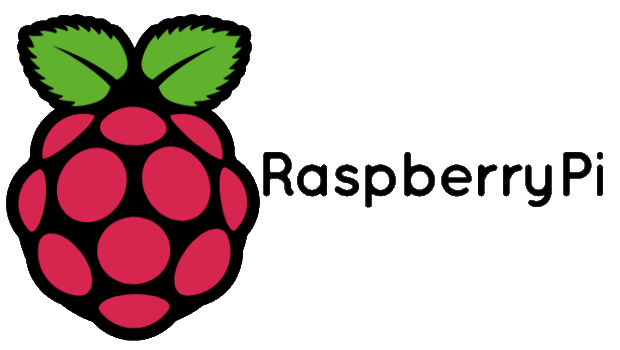
\includegraphics[width=1\textwidth]{raspberry_pi_logo.png}
\end{figure}

Notre première idée a été de faire de la cross-compilation pour compiler notre programme pour Raspberry sous Ubuntu. Il était difficile d'installer le nécessaire, nous avons donc ensuite essayé de compiler directement le projet sur le raspberry. Ceci a entrainé une nouvelle grande phase d'installation : Qt5, Qt-Creator et GStreamer. Malgré quelques difficultés nous avons fini par réussir cette série d'installations ainsi que la compilation. Nous voilà donc avec une application serveur tournant sur le raspberry. Lors du lancement d'un client, le raspberry affiche l'écran reçu et lorsque plusieurs clients se connectent, l'affichage est divisé pour laisser de la place à tous les utilisateurs. Nous sommes pour le moment obligés de passer par un téléphone portable faisant office de routeur car \textbf{Wifi Campus} bloque les ports.

\section{Avancement actuel}

Nous allons récapituler ici ce qui marche pour le moment. Nous avons deux projets Qt-Creator distincts : un client et un serveur. Tous deux compilent avec GStreamer 1.0 et Qt 5, sous Ubuntu et Raspberry. 

Notre serveur écoute sur un port et, lorsqu'il reçoit un message TCP sur son port d'écoute, ouvre une nouvelle socket sur un port différent pour permettre la communication avec le client et l'échange de flux. Lorsque plusieurs clients se connectent en même temps le serveur est capable de diviser la fenêtre pour afficher le nouveau client. Néanmoins, ceci n'est pas fait dynamiquement dans le sens ou l'on doit relancer la fenêtre dans son ensemble. 

Côté client, lors du lancement le programme propose de se connecter à un serveur et envoie ensuite le flux de votre écran. De plus, nous avons mis en place un chat distribué qui serait à améliorer par la suite. Notre interface graphique se limite au minimum car ce n'était pas dans nos objectifs de départ, mais une séparation MCV a été faite pour permettre une amélioration facile ultérieurement.

\section{Évolution}

Il nous reste à implémenter différentes fonctionnalités pour obtenir quelque chose de complet et de fonctionnel. À titre d'exemple, la différenciation entre un élève et un professeur n'est pas faite. Il faudrait avoir une base de données sur le serveur pour que, lors de la connexion, le serveur puisse indiquer au client de quel type il est. Une fois ceci réalisé nous pourrons implémenter les fonctionnalités qui nécessitent la distinction entre les deux types d'utilisateurs.

La fonctionnalité la plus facile à rajouter est le zoom/dezoom sur un écran. Il faudra aussi trouver une meilleure répartition des écrans lors de l'ajout et de la suppression d'un client.

\section{Conclusion}

Il nous reste beaucoup de travail à faire pour réaliser tous les objectifs prévus initalement, mais la base est construite.

\clearpage
\end{document}
